
\documentclass[nooutcomes]{ximera}
%\documentclass[space,handout,nooutcomes]{ximera}

% For preamble materials

\usepackage{pgf,tikz}
\usepackage{mathrsfs}
\usetikzlibrary{arrows}
\usepackage{framed}
\usepackage{amsmath}
%\pgfplotsset{compat=1.16}

\graphicspath{
  {./}
  {algorithms/}
  {../algorithms/}
}

\pdfOnly{\renewenvironment{image}[1][]{\begin{center}}{\end{center}}}

%%% This set of code is all of our user defined commands
\newcommand{\bysame}{\mbox{\rule{3em}{.4pt}}\,}
\newcommand{\N}{\mathbb N}
\newcommand{\C}{\mathbb C}
\newcommand{\W}{\mathbb W}
\newcommand{\Z}{\mathbb Z}
\newcommand{\Q}{\mathbb Q}
\newcommand{\R}{\mathbb R}
\newcommand{\A}{\mathbb A}
\newcommand{\D}{\mathcal D}
\newcommand{\F}{\mathcal F}
\newcommand{\ph}{\varphi}
\newcommand{\ep}{\varepsilon}
\newcommand{\aph}{\alpha}
\newcommand{\QM}{\begin{center}{\huge\textbf{?}}\end{center}}

\renewcommand{\le}{\leqslant}
\renewcommand{\ge}{\geqslant}
\renewcommand{\a}{\wedge}
\renewcommand{\v}{\vee}
\renewcommand{\l}{\ell}
\newcommand{\mat}{\mathsf}
\renewcommand{\vec}{\mathbf}
\renewcommand{\subset}{\subseteq}
\renewcommand{\supset}{\supseteq}
\renewcommand{\emptyset}{\varnothing}
\newcommand{\xto}{\xrightarrow}
\renewcommand{\qedsymbol}{$\blacksquare$}
\newcommand{\bibname}{References and Further Reading}
\renewcommand{\bar}{\protect\overline}
\renewcommand{\hat}{\protect\widehat}
\renewcommand{\tilde}{\widetilde}
\newcommand{\tri}{\triangle}
\newcommand{\minipad}{\vspace{1ex}}
\newcommand{\leftexp}[2]{{\vphantom{#2}}^{#1}{#2}}

%% More user defined commands
\renewcommand{\epsilon}{\varepsilon}
\renewcommand{\theta}{\vartheta} %% only for kmath
\renewcommand{\l}{\ell}
\renewcommand{\d}{\, d}
\newcommand{\ddx}{\frac{d}{dx}}
\newcommand{\dydx}{\frac{dy}{dx}}


\usepackage{bigstrut}


\newenvironment{sectionOutcomes}{}{}

\usepackage{array}
%\setlength{\extrarowheight}{-.2cm}   % Commented out by Findell to fix table headings.  Was this for typesetting division?  
\newdimen\digitwidth
\settowidth\digitwidth{9}
\def~{\hspace{\digitwidth}}
\def\divrule#1#2{
\noalign{\moveright#1\digitwidth
\vbox{\hrule width#2\digitwidth}}}


\title{Operations and Algorithms}
\author{Bart Snapp and Brad Findell}
\begin{document}
\begin{abstract}
Problems about operations and algorithms. 
\end{abstract}
\maketitle


\begin{problem}Explain what it means for an operation $\star$ to be
  \textit{associative}. Give some relevant and revealing examples and non-examples.
\begin{freeResponse}
\begin{hint}
An operation $\star$ is \textit{associative} if $(a\star b)\star c = a\star (b\star c)$ for all values of $a$, $b$, and $c$.  Addition of numbers is associative, as is multiplication.  Subtraction and division are not.  
\end{hint}
\end{freeResponse}
\end{problem} 

\begin{problem}Consider the following pictures:
\begin{image}
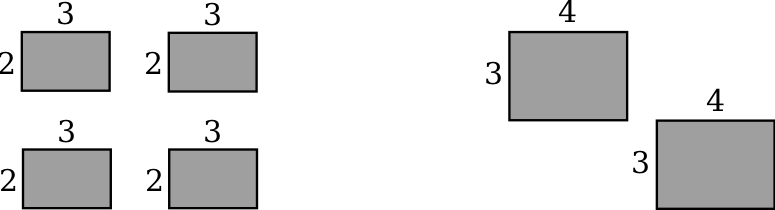
\includegraphics{assMult.png}
\end{image}
Jesse claims that these pictures represent $(2\cdot 3)\cdot 4$ and
$2\cdot (3\cdot 4)$.
\begin{enumerate}
\item Is Jesse's claim correct? 
\begin{multipleChoice}
\choice[correct]{Yes.}
\choice{No.}
\choice{Not enough information.}
\end{multipleChoice}
\item Explain your reasoning.
\begin{freeResponse}
\begin{hint}
Jesse is correct.  The picture on the left is $4$ copies of $2\cdot 3$, and the picture on the right is $2$ copies of $3\cdot 4$.  
\end{hint}
\end{freeResponse}
\item Do Jesse's pictures show the associativity of multiplication? 
\begin{multipleChoice}
\choice{Yes.}
\choice[correct]{No.}
\choice{Not enough information.}
\end{multipleChoice}
\item If so, explain why. If not, draw new pictures representing $(2\cdot
  3)\cdot 4$ and $2\cdot (3\cdot 4)$ that do show the associativity
  of multiplication.
\begin{freeResponse}
\begin{hint}
We can compute that in both cases the total area is $24$, but that does not explain \textit{why} they are the same.  For that, imagine the volume of a box measuring $2$ by $3$ by $4$.  Slicing the layers different ways can explain associativity.  
\end{hint}
\end{freeResponse}
\end{enumerate}
\end{problem} 

\begin{problem}Explain what it means for an operation $\star$ to be
  \textit{commutative}. Give some relevant and revealing examples  and non-examples.
\begin{freeResponse}
\begin{hint}
An operation $\star$ is \textit{commutative} if $a\star b = b\star a$ for all values of $a$ and $b$.  Addition of numbers is commutative, as is multiplication.  Subtraction and division are not.  
\end{hint}
\end{freeResponse}
\end{problem} 

\begin{problem}Explain what it means for an operation $\star$ to \textit{distribute}
  over another operation $\dagger$. Give some relevant and revealing
  examples and non-examples.
\begin{freeResponse}
\begin{hint}
An operation $\star$ \textit{distributes} over an operation $\dagger$ if $a\star(b\dagger c) = (a\star b) \dagger (a\star c)$ and $(b\dagger c)\star a = (b\star a) \dagger (c\star a)$.  
Multiplication distributes over addition because $a\cdot(b+c) = (a\cdot b)+(a\cdot c)$ and $(b+c)\cdot a = (b\cdot a)+(c\cdot a)$.  
But exponentiation does not distribute over addition because $(b+c)\wedge a \ne (b\wedge a)+(c\wedge a)$.
\end{hint}
\end{freeResponse}
\end{problem} 

\begin{problem}Explain what it means for an operation $\star$ to be \textit{closed}
  on a set of numbers. 
\begin{freeResponse}
\begin{hint}
A set is closed under an operation $\star$ if for all $a$ and $b$ in the set, $a\star b$ and $b\star a$ are also in the set.  
\end{hint}
\end{freeResponse}

\begin{problem}
Give some relevant and revealing examples and non-examples.
\begin{freeResponse}
\begin{hint}
The counting numbers are closed under addition and also under multiplication but not under subtraction or division.  The set of even numbers (including $0$ and negatives) are closed under addition, subtraction, and multiplication.  The odd numbers, in contrast, are closed under multiplication but under neither addition nor subtraction.
\end{hint}
\end{freeResponse}
\end{problem}
\end{problem} 

\begin{problem}Sometimes multiplication is described as \textit{repeated
  addition}. Does this explain why multiplication is commutative? If
  so give the explanation. If not, give another description of
  multiplication that does explain why it is commutative.
\begin{freeResponse}
\begin{hint}
Repeated addition by itself does not explain \textit{why} multiplication is commutative.  Instead, use an array model, interpreting $a\cdot b$ as, say, $a$ rows by $b$ columns.  Rotate the array $90^\circ$, and it is clear that $b$ rows by $a$ columns, or $b\cdot a$, must be the same number of objects.  Essentially the same reasoning works with an area model.  
\end{hint}
\end{freeResponse}
\end{problem} 

\begin{problem}
In beginning algebra, simplifying expressions often involves \textit{collecting like terms}.  But why does this work?  Well, the expression $3x+4x$ is equivalent to $(3+4)x$ by the \wordChoice{\choice{commutative}\choice{associative}\choice[correct]{distributive}} property.  And then it is clear that $(3+4)x = \answer{7x}$. \end{problem}

\begin{problem}In a warehouse you obtain $20\%$ discount but you must pay a
  $15\%$ sales tax. Which would save you more money: To have the tax
  calculated first or the discount? Explain your reasoning---be sure
  to use relevant terminology.  In particular, which property 
of which operation(s) do you use?  

\textbf{Solution:}  Build a solution in four steps: 
\begin{enumerate}
\item Use a specific starting price. 
\item Generalize the process of computing a price after a discount (assuming no tax).  
\item Generalize the process of computing a price with tax (assuming no discount). 
\item Generalize the two together. 
\end{enumerate}

To get started, try a specific starting price, say $\$200$.  After the discount, the price would be $\$\answer{160}$.  After the tax, the cost is $\$\answer{184}$.  

Now try the other order.  The original price with tax would be $\$\answer{230}$.  Then with the discount, the cost would be $\$\answer{184}$.  This specific example suggests that the order doesn't matter.  But did we just get lucky?  

\begin{problem}
To compute a price after a $20\%$, discount, suppose the price is $\$p$.  The discount, in terms of $p$, will be $\$\answer{0.2p}$.  So the price after the discount would $p - 0.2p$.  And by the distributive property, this is equal to $\answer{0.8p}$.  In other words, rather than computing the discount and subtracting, we can directly compute the new price by multiplying the original price by $\answer{0.8}$.  This makes sense because with a discount of $20$ percent, the price we pay will be $\answer{80}$ percent of the original price.  
\begin{problem}
To compute a price with $15\%$ tax, suppose the price is $\$p$.  The tax, in terms of $p$, will be $\$\answer{0.15p}$.  So the price with tax would $p + 0.15p$.  And by the distributive property, this is equal to $\answer{1.15p}$.  In other words, rather than computing the tax and adding, we can directly compute the new price by multiplying the original price by $\answer{1.15}$.  This makes sense because with a tax of $15$ percent, the price we pay after tax will be $\answer{115}$ percent of the original price.  
\begin{problem}
Again, let the starting price be $\$p$.  

If we apply the discount and then the tax, we multiply $p$ first by $\answer{0.8}$ and then by $\answer{1.15}$, resulting in the expression $\answer{1.15\cdot 0.8p}$. 

If, on the other hand, we apply the tax and then the discount, we multiply $p$ first by $\answer{1.15}$ and then by $\answer{0.8}$, resulting in the expression $\answer{0.8\cdot 1.15p}$. 

These expressions are equal because of the \wordChoice{\choice{commutative}\choice[correct]{associative}\choice{distributive}} property of \wordChoice{\choice{addition}\choice{subtraction}\choice[correct]{multiplication}\choice{division}}.  Thus, the final cost is the same either way. 
\end{problem}
\end{problem} 
\end{problem}
\end{problem}


\begin{problem}Money Bags Jon likes to give a tip of $20$\% when he is at
  restaurants. He does this by dividing his bill by $10$ and then
  doubling it. Explain why this works.
\begin{freeResponse}
\begin{hint}
Because $10\%$ is the same as $1/10$ of the bill, and $20\%$ is twice that.  
\end{hint}
\end{freeResponse}
\end{problem} 

\begin{problem}Regular Reggie likes to give a tip of $15$\% when he is at
  restaurants. He does this by dividing his bill by $10$ and then
  adding half more to this number. Explain why this works.
\begin{freeResponse}
\begin{hint}
Because $10\%$ is the same as $1/10$ of the bill, $5\%$ is half that, and $15\%$ is the same as $10\% + 5\%$.  
\end{hint}
\end{freeResponse}
\end{problem} 

\begin{problem}Wacky Wally has a strange way of giving tips when he is at
  restaurants. He does this by rounding his bill up to the nearest
  multiple of $7$ and then taking the quotient (when that new number
  is divided by $7$). Explain why this isn't as wacky as it might
  sound.
\begin{freeResponse}
\begin{hint}
If the bill is already a multiple of $7$, then $1/7$ of the bill is about $14.3\%$, which is slightly less than a standard tip of $15\%$.  By rounding up to the nearest multiple of 7, the tip will alway be at least $14.3\%$ and usually slightly more.  
\end{hint}
\end{freeResponse}
%% \begin{teachingnote}
%% The problem above is fundamentally different than the other (related)
%% problems involving tips.
%% \end{teachingnote}
\end{problem} 

%\begin{problem}Cheap Carl likes to give a tip of $13\frac{1}{3}$\% when he is
%  at restaurants. He does this by dividing his bill by $10$ and then
%  adding one-third more to this number. Explain why this works.
%\end{problem} 

%\begin{problem}Reasonable Rebbecca likes to give a tip of $18$\% when she is at
%  restaurants. She does this by dividing her bill by $5$ and then
%  removing one-tenth of this number. Explain why this works.
%\end{problem} 
%
%\begin{problem}Can you think of and justify any other schemes for computing the
%  tip?
%\end{problem} 


\end{document}
